\clearpage
\section{Advanced simulations}

For truly innovative scientific applications, the user is usually forced to
define complex initial conditions, to impose time varying boundary conditions
or to use more than the 5 standard Euler variables (chemical species for
example).  We briefly describe the easiest way to do it in RAMSES.

\subsection{Patching the code}

The general philosophy to design advanced RAMSES applications is to ``patch the
code''. What do we mean by that? A few key routines have been designed in
RAMSES in a user-friendly fashion, allowing the user to edit the file,
modify it according to it needs and recompile the code. For that, it is
recommended to create your own directory, for example \cmd{mypatch/}, in which
you will copy the various files you plan to modify. In the \cmd{Makefile}, you
need to specify the complete path of this directory in the \cflag{PATCH}
variable, as:
%
\begin{Prompt}
PATCH=/home/foo/mypatch  
\end{Prompt}
%
The \cmd{make} command will seek for sources files in this directory first,
compile and link them if present. If not, it will use the default source
files already available in the RAMSES package. Virtually any RAMSES source file
can be modified to obtain a ``patched'' version of RAMSES that fulfill your
needs. Usually, however, only a few routines need to be modified in order to
perform advanced simulations.  These routines will be described now in more
detail. The corresponding files are stored in various RAMSES subdirectories.
These are: \cmd{amr/units.f90}, \cmd{hydro/boundana.f90},
\cmd{hydro/condinit.f90}, \cmd{poisson/gravana.f90},
\cmd{poisson/rho\_ana.f90}, \cmd{hydro/cooling\_fine.f90}. Of course, other
routines of RAMSES can be modified at will, although potential changes might be
more complicated to implement. A simple example of patch can be found in the
directory \dir{patch/} of the package. 

\subsection{Physical units}

This very simple routine can be found in directory \dir{amr/} and is called
\cmd{units.f90}. It is used to set the conversion factors from the user units
into the cgs unit system. In this routine, the user must provide 3 scaling
factors, namely \cmd{scale\_d} for the density units in
$\mathrm{g}.\mathrm{cm}^{-3}$, \cmd{scale\_l} for the length scale in cm and
\cmd{scale\_t} for the time scale in seconds. For self-gravity runs, since
RAMSES assumes $G=1$ in the Poisson equation, it is mandatory to define the
time scale as \cmd{scale\_t=1.0/sqrt(G*scale\_d)} with \cmd{G=6.67d-8}. These
scaling factors are stored in the output files and can be used later on during
post-processing.

\subsection{Initial conditions}

This routine can be found in directory \dir{hydro/} and is called
\cmd{condinit.f90}. It is self-documented. The calling sequence is just
\cmd{call condinit(x,u,dx,ncell}), where \cmd{x} is an input array of cell
center positions, \cmd{u} is an output array containing the volume average of
the fluid conservative variables, namely ($\rho$, $\rho u$, $\rho v$, $\rho w$
and $E$), in this exact order. If more variables are defined, using the
\cmd{-D\cflag{NVAR}} directive, then the user should exploit this routine to
define them too. \cmd{dx} is a single real value containing the cell size for
all the cells and \cmd{ncell} is the number of cells.  This routine can be used
to set the initial conditions directly with Fortran instructions. Examples of
such instructions can be found in directory \dir{patch/}.

Another way to define initial conditions in RAMSES is by using input files. For
the hydro solver, these files are always in the \pkg{grafic} format. We have
already explained how to use the \pkg{grafic} format for cosmological runs. For
non-cosmological runs, initial conditions can be defined using the exact same
format, except that instead of 4 files (\cmd{ic\_deltab}, \cmd{ic\_velbx},
\cmd{ic\_velby} and \cmd{ic\_velbz}), one now needs 5 files called
(\cmd{ic\_d}, \cmd{ic\_u}, \cmd{ic\_v}, \cmd{ic\_w} and \cmd{ic\_p}) and
containing the fluid primitive variables.

For collisionless particles, the \pkg{grafic} format is used only for
cosmological runs, for which particles are initially placed at the cell centers
of a Cartesian grid. For non-cosmological runs, the particles' initial
positions, velocities and masses are read in an ASCII file, in which each line
corresponds to one particle, and should contain the following particle
attributes: \cmd{x,y,z,vx,vy,vz,m}.

\subsection{Boundary conditions}
\label{sec:bc}

As explained in the previous sections, RAMSES can provide boundary conditions
of different types: periodic (default mode), reflexive, outflow and imposed.
This is performed in RAMSES using ghost regions, in which the fluid variables
are set in order to obtain the required boundary. Ghost regions are defined in
the namelist block \nmlblock{\&BOUNDARY\_PARAMS}. Each region is identified by
its position, its type and eventually by the value of the fluid variables. 

\begin{warning}
The exact order with which boundary regions are entered in the namelist block
is very important. Let us consider the 4 boundary regions shown in figure
\ref{fig:bc}. They are defined by the following namelist block:
%
\begin{Prompt}
&BOUNDARY_PARAMS
nboundary=4
ibound_min=-1,+1,-1,-1
ibound_max=-1,+1,+1,+1
jbound_min= 0, 0,+1,-1
jbound_max= 0, 0,+1,-1
bound_type= 1, 1, 1, 1
/
\end{Prompt}
%
The first region is located in the rectangle defined by coordinate
$(i=-1,j=0)$, while the third region is defined by coordinates $(-1 \leq i \leq
+1, j=+1)$. The boundary type for all 4 regions is set to ``reflexive''
(\cmd{\nmlentry{bound\_type}=1}). The fluid variables within the ghost region
are therefore taken equal to the values of their symmetric cells, with respect
to the boundary. This is why the order of the ghost regions is so important:
regions 1 and 2 are updated first, using only the fluid variables within the
computational domain.  Regions 3 and 4 are updated afterwards, using the fluid
variables within the computational domain, but also within regions 1 and 2. In
this way, all cells within boundary regions are properly defined, especially in
the 4 corners of the computational domain.
\end{warning}

It is possible to define only 2 regions (say regions 1 and 2 in figure
\ref{fig:bc}), the orthogonal direction will be considered as periodic. For
gravity runs, the gravitational force is also updated in the ghost regions,
following the same rules as the velocity vector.

\begin{figure}
   \begin{center}
   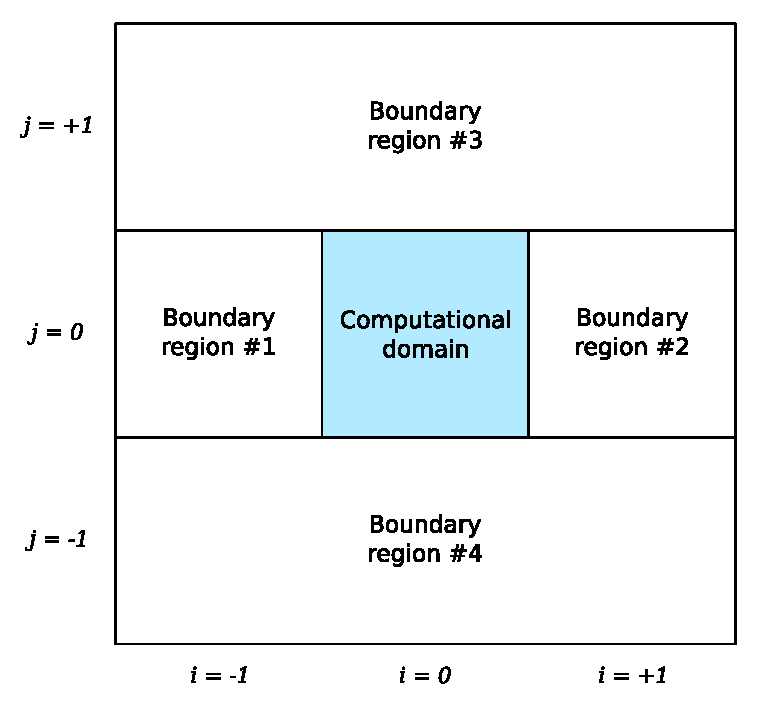
\includegraphics[width=0.65\textwidth]{img/bc.pdf}
   \end{center}
   \caption{Example of ghost regions used in RAMSES to impose specific boundary
conditions.}
   \label{fig:bc}
\end{figure}

For the Poisson equation, however, boundary conditions are either periodic, if
no ghost regions are defined in the corresponding direction, or ``$\phi=0$''
Dirichlet boundary conditions within ghost regions. No other types of boundary
conditions for the Poisson equation have been implemented (such as isolated,
reflexive and so on). 
% TODO update?

If \cmd{\nmlentry{bound\_type}=3}, boundary conditions must be imposed by the
user. The first possibility is to use parameters \nmlentry{d\_bound},
\nmlentry{u\_bound}{\dots} to set a constant fluid state within the desired
ghost region. For more advanced applications, the user is encouraged to patch
the routine \cmd{boundana.f90} within directory \cmd{hydro/}. This routine is
very similar to routine \cmd{condinit.f90}. The calling sequence is \cmd{call
boundana(x,u,dx,ibound,ncell}). The ghost region number is therefore provided,
so the user can specify some region-dependent fluid conditions.

\subsection{External gravity sources}

If \cmd{\nmlentry{bound\_type}=3}, boundary conditions must be imposed also for
the gravitational force. This is performed by modifying routine
\cmd{gravana.f90} in directory \dir{poisson/}. If \cmd{gravity\_type>0}, this
routine is also used to specify the gravitational force within the
computational domain. Note that in this case, the fluid is not self-gravitating
anymore. There is another way to impose an external gravity source and in the
same time, to solve for the Poisson equation. This is done using routine
\cmd{rho\_ana.f90} in directory \dir{poisson/}. In this routine, again very
similar to the previously presented Fortran routines, the user can specify the
density profile for the external gravity source.  This density profile will be
added to the fluid density as the source term in the Poisson equation.

\subsection{External thermal sources}

The final routine that can be easily modified by the user is
\cmd{cooling\_fine.f90} in directory \dir{hydro/}. This routine is used if
\cmd{\nmlentry{cooling}=.true.} or if the polytropic temperature
\cmd{\nmlentry{T2\_star}>0.0}. In the first case, cooling and heating source
terms are added to the energy equation and solved by a fully implicit
integration scheme. In the second case, the thermal energy of the fluid is not
allowed to be lower than a polytropic Equation-Of-State, for which one has $ T
/ \mu = {(T / \mu)}_{*} {(\rho / \rho_{*})}^{\gamma_{*}-1} $.  All starred
parameters can be set within the namelist block \nmlblock{\&PHYSICS\_PARAMS}.
On the other hand, the user might want to modify routine
\cmd{cooling\_fine.f90} in order to implement more complex thermal modeling of
the fluid.

